% !TeX spellcheck = en_US
% !TeX encoding = UTF-8
% !TeX root = ../document.tex

\chapter{Model Unspecific Search}

\section{Motivation}
A collision at an energy of \SI{13}{\TeV} can create a large amount of different particles. Solely by combinatorics, it follows that a lot of different final states are accessible.

Most dedicated searches tend to focus on one or a few final states that represent the signature of the theory under investigation. This leaves many final states not examined, either because of the complexity of the final state or because there is no analysis group currently working on a corresponding theory.

One of the goals of the model unspecific search is to gain knowledge from these additional final states. Additionally, the model unspecific search aims to obtain a global interpretation of the agreement between simulation and observed data across a broad range of final states.

\section{Previous Works}
The approach of a model unspecific search is not a new concept: In 1998, a note about an unspecific search has been written at the L3 experiment (\ac{LEP})\cite{Hebbeker:GlobalComparisonL3}, and in 2004, a similar approach has been applied to data of the D0-experiment at the Tevatron proton-antiproton collider at Fermilab\cite{Biallass:ModelIndependentSearch}.

At \ac{CMS}, the analysis has been developed and regularly applied to observed data since 2009\cite{Schmitz:ModelUnspecificSearch,Hof:ImplementationModelIndependent,Dietz-Laursonn:ModelUnspecificSearch,Olschewski:StudyAlternativeStatistical,Brodski:ModelUnspecificSearch,Pieta:MUSiCModelUnspecific,Papacz:ModelUnspecificSearch,Albert:ExtensionModelUnspecific} \todo{Jonas' Arbeit, Debby und Simon?}. 
This thesis bases on the most recent implementation of the \ac{MUSiC} analysis.\todo{ok so?}

Very recently, the \ac{ATLAS} collaboration published a conference note analyzing \SI{3.2}{\per\femto\barn} of \ac{LHC} data at $\sqrt{s} = \SI{13}{\TeV}$ using a similar model-independent search \cite{ATLAS:ATLAS-CONF-2017-001}. 

\section{Procedure}
As described above (chapter \todo{reference!}), observed data as well as \ac{MC} simulation samples are reconstructed centrally by the \ac{CMS} collaboration. 
As first step of the \ac{MUSiC} analysis, requirements on events and physics objects are applied \todo{reference -> Event/Object selection}, discarding invalid events and extracting objects for the \ac{MUSiC} analysis.
Afterwards, each event is classified sorted into so-called \emph{event classes}, sets of events that share the same final state \todo{ref}.
For each event class, the kinematic variables of each event are calculated and \emph{kinematic distributions} are aggregated.
Up to this point, the same procedure is applied to simulated data and observed data.
Subsequently, an automated search algorithms finds the largest deviation between data and simulation within each kinematic distribution of each event class. Afterwards, the global significance of each deviation is estimated from Standard-Model only simulations.

\section{Event Classes}
An event class is a set of events sharing the same final state. The final state is indicated by the name of the event class: All events in the class named \eventclass{2\Pe + 1\Pmu}, for example, contain two electrons and one muon in the final state.

There are three types of event classes: \emph{exclusive}, \emph{inclusive} and \emph{jet inclusive}.

Events in the exclusive event classes contain exactly the indicated (and no additional) particles in their final state. Each event thus belongs to exactly one exclusive event class.

Inclusive event classes are denoted with the suffix "\eventclass{+ X}" in the name (e.g. \eventclass{2\Pe + 1\Pmu + X}). Their final state contains the explicitly stated particles plus any additional ones. Each event can be assigned any number of inclusive event classes. One advantage of this procedure is a larger number of events per class which can be beneficial \todo{for what?}. However, the correct combination of statistical results across multiple inclusive event classes is not trivial.

Jet inclusive event classes are denoted with the suffix "\eventclass{+ Njets}" in the event class name (e.g. \eventclass{2 \Pe + 1\Pmu + Njets}). Events contained in a jet inclusive event class may contain any number of jets in addition to the explicitly stated objects. This increases the number of events per class, as effects like initial or final state radiation are ignored, leading to reduced statistical uncertainties.

In any case, the kinematic variables are only calculated from the objects explicitly stated in the class name, in our example two electrons and one muon.


\section{Objects}

\subsection{Electrons}

\subsection{Muons}

\subsection{Photons}

\subsection{Jets}

\subsection{Missing Transverse Energy}



\section{Kinematic Variables and Distributions}

\subsection{Sum of Transverse Momenta}

\subsection{Invariant Mass}

\subsection{Missing Transverse Energy}


\section{Search for Deviations}
\label{sec:deviations_search}


\subsection{Search Space}

\subsection{Global Significance}

\newcommand{\sign}{\theta}

The goal of the automated search is to search within each distribution for the region with the largest deviation between expectation and observed data. Then, we calculate the probability $p$ of observing such a deviation somewhere in the distribution, just by chance, taking the \ac{SM} prediction as null-hypothesis.

This procedure of calculating a global $p$-value from a local significance is also called \emph{Bonferroni correction}. Usually, this is done by calculating a correction factor and applying it to the local significance.

In our case, this method is not feasible: Since the probabilities of overlapping regions overlap, we cannot just compute a correction factor by combinatorics. 

Instead, a simulation-based approach of \emph{pseudo-experiments} is used: For each bin of the distribution, a random number is drawn from the probability distribution caused by systematical and statistical uncertainty on the \ac{SM} expectation value. The resulting \emph{pseudo-distribution} is subsequently again compared to the expectation using the described search algorithm, yielding a local significance value $\sign$ for each pseudo-experiment.

\begin{equation}
    \sign_\text{min} = \min(\left\{\text{region}\sign(\text{region}) \forall \text{ region} \in \text{distribution} \right\})
\end{equation}

\begin{equation}
    \p = \frac{\left|\left\{\text{pseudo-experiment} \mid \sign_\text{min}(\text{pseudo-experiment}) < \sign_\text{min}(\text{data}) \right\}\right|}{\left|\left\{\text{pseudo-experiments}\right\}\right|}
    \label{eq:look_elsewhere_correction}
\end{equation}


Within the (statistical and systematical) uncertainty distribution of the Standard Model  


The statistical nature of the Standard-Model is simulated by randomly choosing values for the observed number of events in each bin.




The probabilities of observing deviations are correlated between overlapping regions. 


Since the regions' overlap, the regions are correlated. Thus, the probabilities of observing deviations by chance are correlated between overlapping regions.

assess the significance of a deviation, expressed as probability to observe a deviation the same as or more extreme just by chance (given SM) SOMEWHERE in the distribution

procedure also known as Bonferroni correction

correction factor cannot be calculated analytically because of correlations between regions

idea: pseudo-experiment, simulate circumstances using SM only, count more-extreme values, interpret fraction as probability (frequentist  approach)

problem: need measure for "extremity" of deviation (-> also used for finding RoI)





\subsection{Significance Estimator}
measure "extremity" of deviation (-> for finding RoI as well as global correction)

choice is ambiguous

choice: value interpretable as probability for local deviation

back to definition: sum of probabilities of more extreme events

start using Poissonian probability
include Gaussian prior: either normal or log normal


\subsection{Treatment of Regions with Low \ac{MC} Event Numbers}


\subsection{Look-Elsewhere-Effects}
\subsubsection{Regions}
corrected using global significance 

\subsubsection{Classes}
\subsubsection{Distributions}

\section{Implementation}
\subsection{Software Environment}
CMSSW, ROOT, Python/C++

\subsection{Analysis Framework}
Skimming, Pxl, TAPAS, MUSiC

\subsection{MUSiC Workflow}

\subsection{Automation}
\begin{figure}
    \centering
    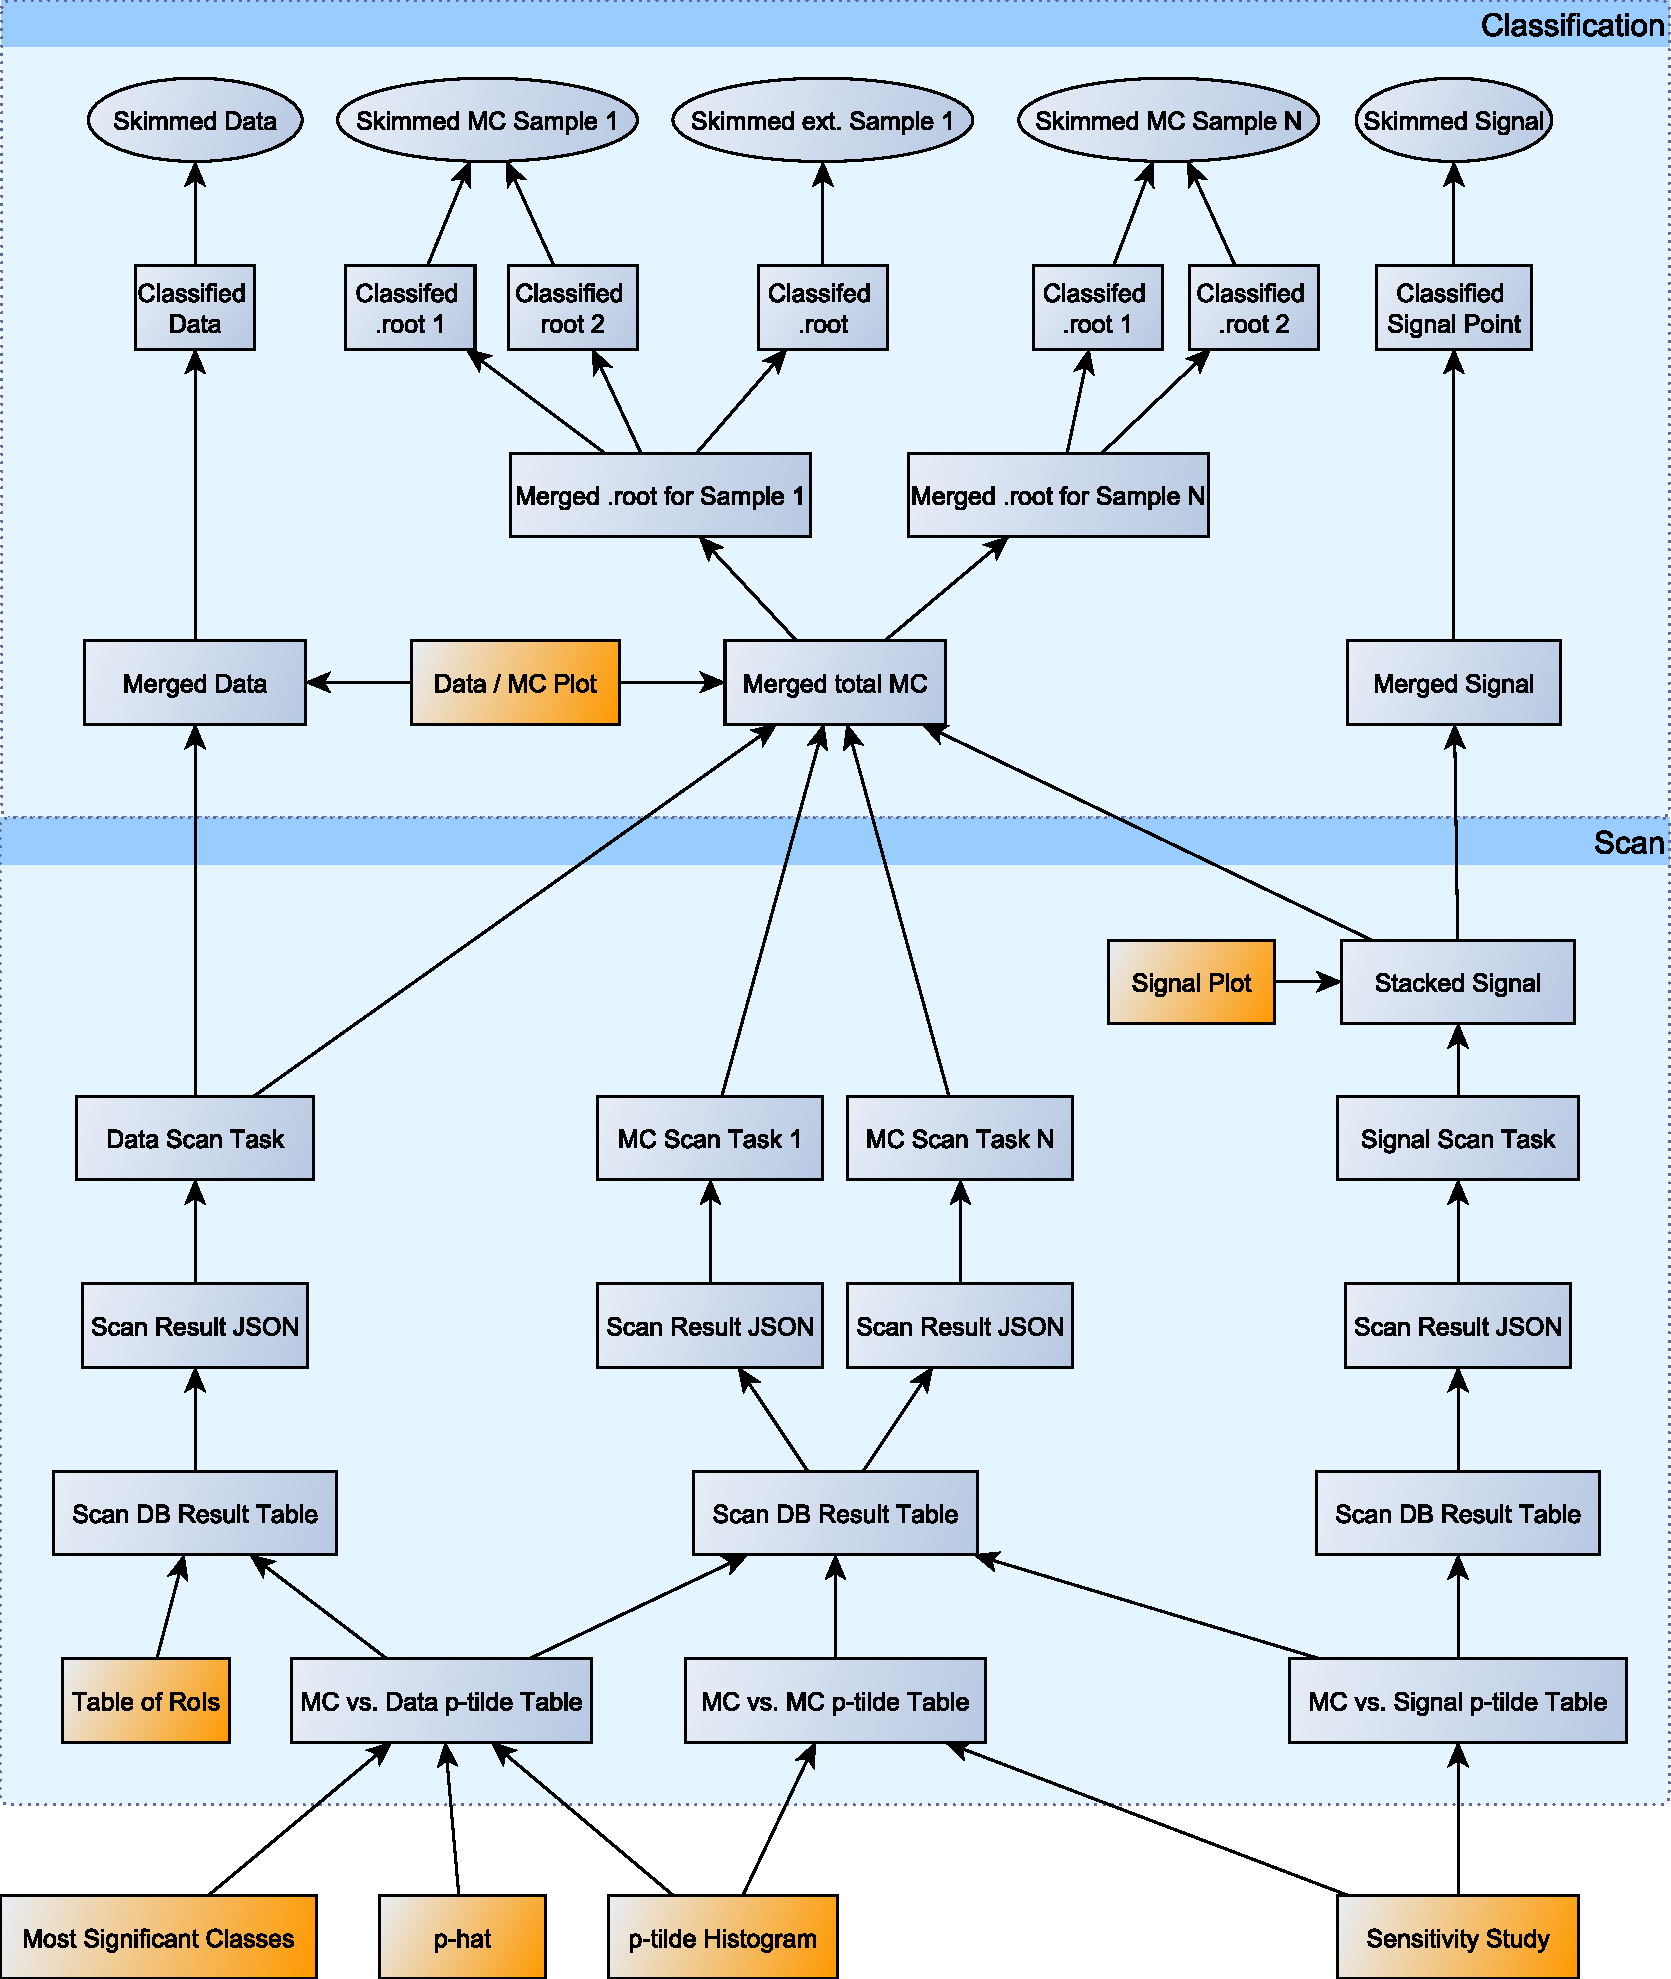
\includegraphics[width=\textwidth]{../music-workflow}
    \vspace{0.5em}
    \caption{Implementation of the MUSiC-Workflow. Using the Luigi-Automation Framework, these steps are performed on demand.}
    \label{fig:music_workflow}
\end{figure}

Luigi